\chapter{Theory}

This chapter introduces the PCG algorithms and concepts considered throughout the report and ends with an introduction to relevant fundamentals of 3D graphics.
The PCG-related subchapters are roughly ordered by how frequently their concepts occur in PCG research, starting with the most common ones.

\section{Noise}

Noise is one of the most fundamental concepts of PCG and there exists several flavors of it.
The two major types of noise are \textit{value noise} and \textit{gradient noise}, which can both be expressed using the following function.
$$
  f(\vec x) = y \in [0, 1] \text{ where }
  y \in \mathbb{R},
  \vec x \in \mathbb{R}^n,
  n \in \mathbb{Z}^+
$$
This function is deterministic, but the output for any single input is perceived as random.
This is achieved by combining a Random Number Generator (RNG) with an interpolation function.
The way that these two functions are implemented and utilized is what differs value noise from gradient noise.

Value noise is constructed by first randomizing the values of all lattice points in an $n$-dimensional space using an RNG function.
These points are then interpolated to define intermediate points, resulting in a continuous $n$-dimensional space of random values.
The noise function then simply outputs the real number defined at coordinate $\vec x$ within this space.
The interpolation function used is typically bilinear or bicubic in the setting of real-time computer graphics, as they are computationally cheap.

Although simple to implement, value noise has several disadvantages.
First off, the resulting noise has a visually grid-like structure.
This is often undesired in graphics since it creates arbitrary patterns in the noise.
Moreover, neighboring lattice points sometimes greatly differ in values which can result in sudden changes in intensity.

Gradient noise solves the major problems present in value noise by randomizing $n$-dimensional gradient vectors at each lattice point, instead of real numbers.
This modification ensures that the interpolated values have smooth continuous gradients (i.e. partial derivatives) and not just smoothly interpolated values.

Some common implementations of gradient noise include \textit{Perlin noise} \cite{perlin_noise} \cite{perlin_noise2}, \textit{Simplex noise} \cite{simplex_noise}, and \textit{OpenSimplex noise} \cite{opensimplex_noise_blog} \cite{opensimplex_noise_code}.
Ken Perlin originally invented Perlin noise with the intention to produce more natural-looking textures \cite{perlin_noise}, and later invented Simplex noise to address some of the limitations with Perlin noise \cite{simplex_noise}.
Usage of Simplex noise is however restricted due to its patent \cite{opensimplex_noise_patent}.
Fortunately, Kurt Spencer invented a well-performing variation called \textit{OpenSimplex noise} which was released into the public domain \cite{opensimplex_noise_blog} \cite{opensimplex_noise_code}.
The details of these algorithms are beyond the scope of this paper, but further reading of Perlin noise can be found in the original paper \cite{perlin_noise}, and the ideas behind Simplex noise are described in great detail by Stefan Gustavson in his paper \textit{Simplex noise demystified} \cite{simplex_noise_explained}.

In practice it is common to use a Fractional Brownian Motion (fBm) implementation, which can be constructed by summing noise functions of different amplitudes and sampling frequencies.
The variation in frequency and amplitude between these functions are sometimes referred to as lacunarity and gain respectively.
The usage of fBm allows for greater control over the resulting noise function's visual properties, making it more suitable for many applications in computer graphics.

\begin{figure}[h!]
  \centering
  \begin{subfigure}[b]{0.30\textwidth}
    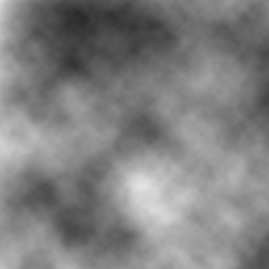
\includegraphics[width=\textwidth]{figure/value_noise.png}
    \caption{Value noise. \cite{value_noise_img}}
  \end{subfigure}
  \quad
  \quad
  \quad
  \begin{subfigure}[b]{0.30\textwidth}
    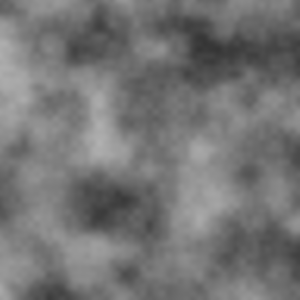
\includegraphics[width=\textwidth]{figure/perlin_noise.png}
    \caption{Gradient noise. \cite{perlin_noise_img}}
  \end{subfigure}

  \caption{Examples of value noise and gradient noise represented using intensity maps. Notice how the value noise has cross-like patterns.}
  \label{fig:noisetypes}
\end{figure}

The output of noise functions can be visualized in many ways, intensity maps being one of them (see figure~\ref{fig:noisetypes}).
An intensity map is a bitmap image where each pixel represents the value of the underlying noise.
Bright pixels represent high values, while dark pixels represent low values.
These maps can be used to represent various things such as heights, in which case they are referred to as \textit{heightmaps}.
They can also be used to blend textures together, which is called \textit{texture splatting}.
\section{L-Systems}

Another fundamental concept in PCG is L-systems.
An L-system is a type of formal grammar where all symbols are evaluated in parallel.
It is built up of strings which under a set of constraints recursively grow larger and more complex with each iteration.
These strings can then used to generate complex geometric structures, often with factorial properties.
The technique's inventor, Aristid Lindenmayer originally used it to model a wide array of plants \cite{lsystem_book}.
L-systems are formally defined by three parameters which can be denoted as follows:

\begin{itemize}
  \item V  - The alphabet, consists of replaceable symbols (variables or non-terminals) and static symbols (constants or terminals).
  \item $\omega$ - The axiom, an initial variable from V which defines the initial state.
  \item P - The production rules, these are the constraints which determine how variables should be replaced.
\end{itemize}

For instance, $G(V, \omega, P) = (\{A, B\}, A, \{(A \to AB), (B \to A)\})$ would produce
\begin{align*}
  n &= 0: A \\
  n &= 1: AB \\
  n &= 2: ABA \\
  n &= 3: ABAAB \\
  n &= 4: ABAABABA \\
  &\dots
\end{align*}

for the first 4 evaluation iterations. The symbols of the resulting string can then be interpreted as different actions.
The above example could be used to build a corridor where A represents empty space and B represents a door.

There is a special case of L-systems which is called \textit{Stochastic bracketed L-systems}.
Stochastic means that all production rules have a probability of being used for an evaluation, which implies that multiple rules can target the same source string.
Bracketed means that we have a stack structure where the '\textbf{[}' symbol pushes the current state, and '\textbf{]}' pops and restores the previously pushed state.

By being able to return to a previous state, one can produce content with non-continuous generation.
This is well expressed in the book \textit{Procedural Content Generation in Games}~\cite[p.77]{pcg_in_games}, where the authors describe the limitations of non-bracketed L-systems in the following way:
\begin{center}
“While interpreting L-system-generated strings as turtle instructions allow us to draw complex fractal shapes, we are fundamentally limited by the constraint that the figures must be drawable in one continuous line—the whole shape must be drawn 'without lifting the pencil'”. 
\end{center}

The ideas from L-systems can also be extended beyond strings, with some examples being Shape grammars \cite{shape_grammars} and Graph grammars \cite{graph_grammars}.
Graph grammars use graphs from discrete mathematics instead of letters.
This difference enables graph grammars to produce non-sequential graph results, as opposed to 1-dimensional strings, making them suitable for generating quests and level layout.
Unfortunately, this feature also makes them more difficult to implement and more expensive to process than L-systems.
Shape grammars are similar, but operate on geometrical objects instead, making them suitable for Computer-aided Architectural Design (CAAD).
\section{Search-based PCG}

For some generation purposes it can be challenging to precisely describe desired results, but easier to describe desired properties and to compare alternative results.
A suitable technique for handling these situations is Search-based PCG (SBPCG).

SBPCG is a collection of stochastic search algorithms that are combined with domain-specific evaluation functions to iteratively optimize some content \cite{search_based_pcg} \cite{search_based_pcg2}.
Traditionally such search has primarily been performed using Evolutionary Algorithms (EA) such as the $\mu + \lambda$ evolution strategy (ES) \cite[p.18-20]{pcg_in_games}, and NSGA-II \cite{nsgaii}.

SBPCG via EAs is typically done in the following way.
\begin{enumerate}
  \item Manually create or randomize a population of initial content candidates.
  \item Evaluate all candidates with evaluation functions.
  \item Maintain only the best performing candidates and discard the rest.
  \item Search for new candidates similar to the current population. This step typically involves several mutations and crossover operations.
  \item Repeat from step 2, unless current candidates are satisfactory.
\end{enumerate}

The core idea of this process is based on natural selection.
There is a population of individuals (candidates) in each generation that are evaluated, and the fittest (highest evaluated) individuals get the chance to reproduce, while those least fit are removed.
The evaluation of individuals may depend on multiple properties and in PCG it is often desired to maintain diversity in the population as well.
Diversity is important to avoid local maximums, but also to ensure results have enough variation.

Machine Learning (ML) is another method that can be used instead of EAs, in which case the generation is often referred to as Procedural Content Generation via Machine Learning (PCGML) \cite{pcgml} \cite{pcgml2} \cite{pcgml3}.
In PCGML the idea is to generate new content based on patterns found from analyzing existing content by using Artificial Neural Networks (ANN).
This technique is especially effective when large amounts of quality content already exists.
For instance, PCGML could be used to extract patterns from existing bridges in order to combine these patterns to form new bridges.
The main drawback is that such well-structured data of quality content can be difficult to obtain.

There are three main cateogries to consider when deciding on what evaluation functions to use, and these categories are \textit{direct}, \textit{simulation-based}, and \textit{interactive} \cite[p.5-7]{search_based_pcg}.
In direct evaluation, content quality is determined directly by its properties such as size and weight.
In simulation-based evaluation, the interaction between the content and some artificial agent is judged instead.
Finally, in interactive evaluation a human is employed to interact with the generated content.
The human then either explicitly answers what content they preferred, or such feedback is extracted implicitly from gameplay data.

\section{Voronoi Diagrams}

Voronoi diagrams is a technique used to partition a plane into $n$ regions (called Voronoi cells).
This is done by first scattering $n$ nodes, referred to as \textit{seeds}, onto the plane.
Subsequentialy, each seed is assigned its own region and all points on the plane will be assigned to the region of the closest seed.
These regions can then be used in PCG-scenarios such as dividing land areas into regions with less obvious patterns than those formed by using a simple grid.
Another use case is to reduce memory consumption through seamless chunk loading, not unlike \textit{Minecraft} \cite{minecraft}.

\begin{figure}[H]
  \centering
  \begin{subfigure}[b]{0.4\textwidth}
    \frame{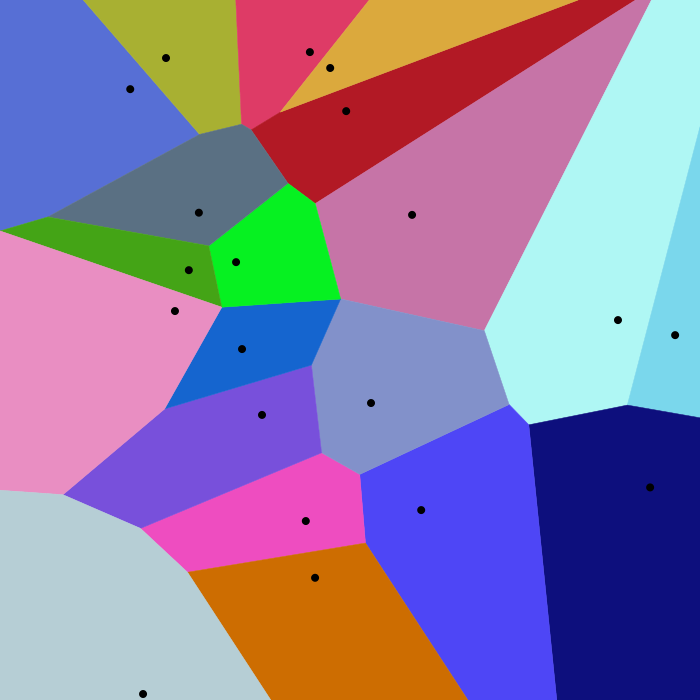
\includegraphics[width=\linewidth]{figure/voronoi_euclidean.png}}
    \caption{Voronoi diagram using Euclidean distance \cite{voronoi_euclidean}.}
    \label{fig:voronoi_euclidean}
  \end{subfigure}
  ~
  \begin{subfigure}[b]{0.4\textwidth}
    \frame{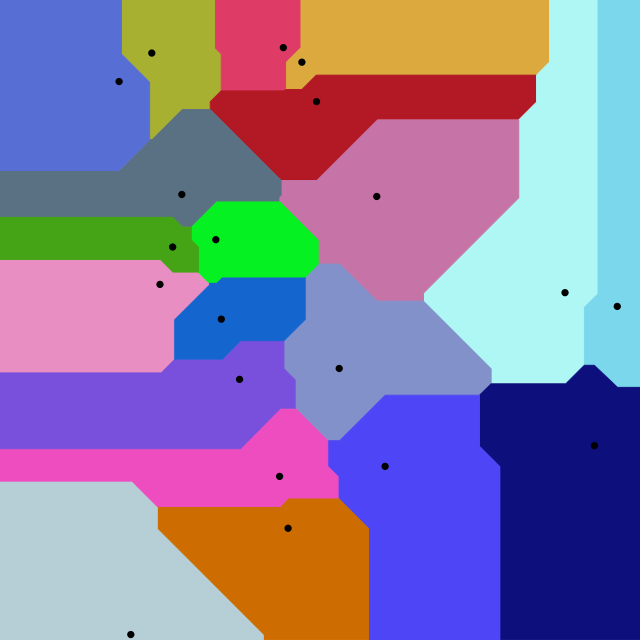
\includegraphics[width=\linewidth]{figure/voronoi_manhattan.png}}
    \caption{Voronoi diagram using Manhattan distance \cite{voronoi_manhattan}.}
    \label{fig:voronoi_manhattan}
  \end{subfigure}
  \caption{Voronoi diagrams using identical seeds but different distance metrics.}
  \label{fig:voronoi}
\end{figure}
\vspace{-0.5cm} % Bad practice

Voronoi diagrams can be visualized by marking seeds with black dots and by coloring each regions' points with an unique color (see examples in figure \ref{fig:voronoi}).
The construction of these diagrams can be implemented using either Lloyd's Algorithm \cite{voronoi_lloyd}, or Fortune's Algorithm \cite{voronoi_fortune}. 
\section{Poisson Disc Sampling}

Poisson Disc Sampling randomizes the placement of points in an $N$-dimensional space such that all points form a single cluster, while maintaining a minimum distance between points.
This algorithm can be implemented in linear time \cite{poisson_fast}, and can be used for randomly placing clusters of trees and shrubs.

% Figure here would be nice.

The idea behind the algorithm is to specify a minimum distance $R$, a sample limit $k$, and then place an initial \textit{active point} in a random position.
Thereafter, the following procedure is repeated until there are no more active points remaining.
\begin{enumerate}
  \item Sample an active point, $P$.
  \item Place up to $k$ new points inside the $[R, 2R]$ annulus centered at $P$.
  \item For each new point,
  \begin{enumerate}
    \item Remove it, if it is within $R$ radius of another point.
    \item Otherwise, add it to the list of active points.
  \end{enumerate}
  \item Mark $P$ as an \textit{inactive point}.
\end{enumerate}

A depth-first variant of the above procedure has been visualized by Mike Bostock, and its JavaScript implementation has been made open-source \cite{poisson_demo}.

In some scenarios it is desired to place objects of various sizes together.
In the case of a forest, one might want to have trees, bushes, and grass for instance.
Blomqvist et al. showed that such placement could efficiently be done by separating objects of different sizes into layers, and then process the generation of each layer in decreasing order of $R$ \cite[p.32]{ba_landscape}.
By applying this hierarchy one avoids the problem of packing small objects so tightly that no room is left for larger objects.
Instead, large objects such as trees get priority, and then smaller objects such as grass can be generated in-between.
\section{Basics of 3D Graphics}

Everything in modern computer graphics is centered around polygon meshes.
A polygon mesh is a geometric graph combined with a set of geometrical faces that together form a surface.
Typically these faces are triangles, in which case the meshes are also referred to as triangle meshes, or simply meshes.
An example of such a mesh is shown in Figure~\ref{fig:low_poly_dolphin}.

\begin{figure}[h!]
  \centering

  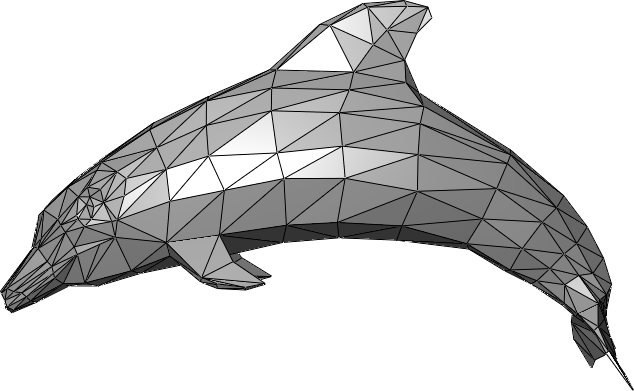
\includegraphics[width=0.5\textwidth]{figure/low_poly_dolphin.png}
  \caption{Example of a low poly triangle mesh representing a dolphin \cite{low_poly_dolphin}.}

  \label{fig:low_poly_dolphin}
\end{figure}

\newpage
Each vertex can store arbitrary data alongside its own coordinates in space.
Examples of such data include: an averaged normal of its neighboring faces, color, reflectance, bone weights and texture coordinates (a.k.a. UV coordinates).
These stored properties can then be used to help compute realistic lighting, colors, animations, and more.

Nowadays it is common to apply high-quality images to meshes, rather than just colors and lighting shades.
Applying these images can be done via a process called \textit{texture mapping} or \textit{UV mapping}, which entails designing 2D textures and mapping these onto 3D meshes using the UV coordinates of the vertices.
An example of this process can be found in Figure~\ref{fig:uv-mapping}.

\begin{figure}[h!]
  \centering
  \begin{subfigure}[b]{0.30\textwidth}
    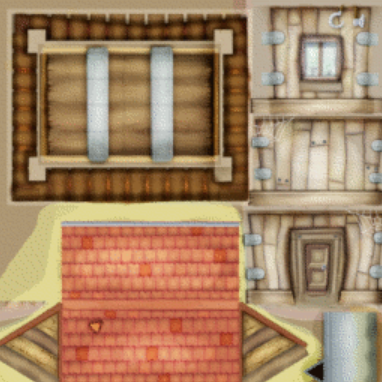
\includegraphics[width=\textwidth]{figure/uv-mapping1.png}
    \caption{House texture map.}
  \end{subfigure}
  \quad
  \quad
  \quad
  \begin{subfigure}[b]{0.30\textwidth}
    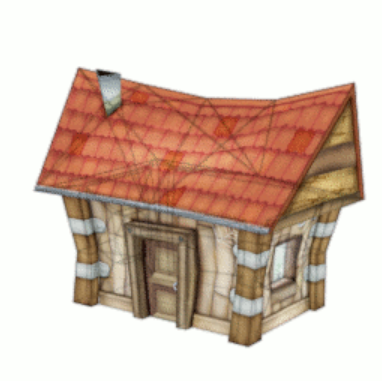
\includegraphics[width=\textwidth]{figure/uv-mapping2.png}
    \caption{Textured house mesh.}
  \end{subfigure}

  \caption{Example of UV mapping a texture map onto a model of a house \cite{house_uv_mapping}. Notice how UV coordinates are reused to apply the same texture to each pillar.}
  \label{fig:uv-mapping}
\end{figure}

Models can be future enhanced by using materials and shaders.
A material contains all the visual properties of a model except for the mesh itself.
This may include multiple constants, textures, and shaders.
Shaders are programs designed to run on GPUs and can be used to combine textures in various ways to create interesting visual effects.
The downside is that shaders are typically strongly tied to specific software or hardware, making them difficult to port.
Consequently, standard file formats for 3D models such as \textit{.obj}, \textit{.fbx}, and \textit{.gltf} have limited support for shaders.


% TODO: The stuff below should probably get their own subchapters.
% genotype, phenotype, Spelunk and Occupancy Regulated Extension (OCE): https://www.researchgate.net/publication/221157490_Procedural_level_generation_using_occupancy-regulated_extension
% Unexplored and Cyclic Dungeon Generation (article source https://ctrl500.com/tech/handcrafted-feel-dungeon-generation-unexplored-explores-cyclic-dungeon-generation/)(park source https://www.youtube.com/watch?v=mA6PacEZX9M)
% WaveFunctionCollapse
